%%%%%%%%%%%%%%%%%%%%%%%%%%%%%%%%%%%%%%%%%%%%%%%%%%%%%%%%
%%%%%%%%%%%%%%%%%%%%%%%%%%%%%%%%%%%%%%%%%%%%%%%%%%%%%%%%
\section{Unsupervised Learning}
\label{additional:unsupervised}

%%%%%%%%%%%%%%%%%%%%%%%%%%%%%%%%%%%%%%%%%%%%%%%%%%%%%%%%
\subsection{Bayesian Optimization}
\label{additional:unsupervised:BO}

Frequently we are fortunate enough to have a fairly explicit form of
the objective function $S\left(\bm{\beta}\right)$ to be optimized in order to solve a problem.
However, when $S\left(\bm{\beta}\right)$ is not well-known,
is expensive to compute\footnote{The performance of a machine learning model as a function of its hyperparameters is a classic example of this.
In that case, evaluating $S$ amounts to training the model with a particular set of hyperparameters $\bm{\beta}$,
then determining it's performance on a metric such as ROC AUC.}, or is non-differentiable,
the usual gradient based approaches, such as SGD and Newton's method, break down.
In these cases ``black box''\footnote{Black box as in
we do not have a closed-form expression for $S$, or know $\grad S$.} methods\footnote{Other examples of black box optimizers include
Tree-Structured Parzen Estimators (TPE),
genetic algorithms,
and some additional tree based methods described in \cite{Hutter2011,Hutter2014}.
A TPE is a close relative of Bayesian optimization, making use of the opposite side of Bayes' theorem by
estimating $P\left(\bm{\beta} \mid S\right)$ and $P\left(S\right)$ rather than $P\left(S \mid \bm{\beta}\right)$.
TPEs can accommodate categorical $\beta_{i}$ in a hierarchical manner,
however they can not model interactions between the $\beta_{i}$ \cite{bissuel_2019,NIPS2011_4443}.},
such as Bayesian optimization, may be used instead.

In Bayesian optimization\footnote{Generalized
formally as Sequential Model-Based Optimization (SMBO) \cite{NIPS2011_4443}.} \cite{Brochu2010,1301.1942,Borisyak,NIPS2011_4443},
$S$ is approximated by a well-known surrogate function\footnote{Also known as a response surface.}.
The surrogate typically is a Gaussian process (GP),
but can be any well-behaved regressor such as
a Random Forest or Boosted Decision Tree (BDT).
GPs \cref{eq:additional:unsupervised:BO:GP} are
extensions of Gaussian distributions which return a Gaussian at any point along their domain.
They are parameterized by a mean function\footnote{For convenience,
the prior $m\left(\bm{x}\right)$ is usually assumed to be zero, $m\left(\bm{x}\right)=0$.}, $m\left(\bm{x}\right)$,
and covariance function, $k\left(\bm{x}_{i}, \bm{x}_{j}\right)$,
\ie kernel\footnote{The kernel of the GP is a hyperparameter to be chosen in advance.
Standard kernel choices include
the radial basis function kernel $k\left(\bm{x}_{i}, \bm{x}_{j}\right) = \exp\left(-\frac{1}{2\sigma^{2}}\norm{\bm{x}_{i}-\bm{x}{j}}^{2}\right)$,
Mat\'{e}rn kernel,
and white noise kernel $k\left(\bm{x}_{i}, \bm{x}_{j}\right) \propto \delta_{ij}$.},
instead of a constant mean $\mu$ and variance $\sigma^{2}$.
An illustration of a GP is provided in \cref{fig:additional:unsupervised:BO:GP_ex}.

\begin{equation}\label{eq:additional:unsupervised:BO:GP}
f\left(\bm{x}\right) \sim \mathcal{GP}\left(m\left(\bm{x}\right), k\left(\bm{x}_{i}, \bm{x}_{j}\right)\right).
\end{equation}

\begin{figure}[H] % TODo might want to eventually remove
\centering
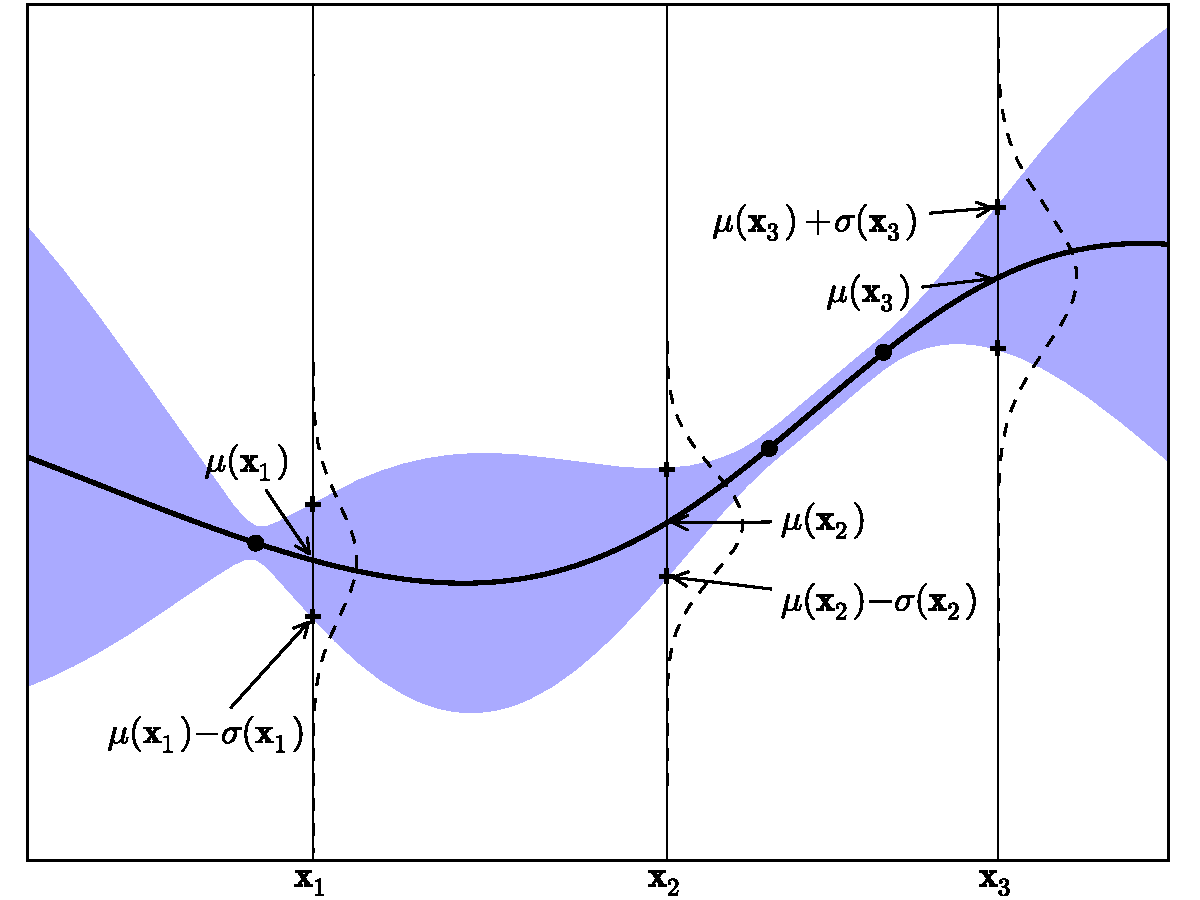
\includegraphics[width=0.85\textwidth]{figures/ml/gp.pdf}
\caption{
Illustration of a Gaussian process (GP) in 1D \cite{Brochu2010}.
Note that at any point $\bm{x}_{1}$, $\bm{x}_{2}$, $\bm{x}_{3}$ the GP
returns a Gaussian distribution characterizing the estimated mean and uncertainty on the
unknown true function, \ie the objective function $S\left(\bm{\beta}\right)$ in the case of Bayesian optimization.
}
\label{fig:additional:unsupervised:BO:GP_ex}
\end{figure}

The surrogate function is initially fit to
a random sample of $\bm{\beta}$, $S\left(\bm{\beta}\right)$ points.
From this prior, Bayesian optimization
operates by iteratively sampling $S\left(\bm{\beta}\right)$ and updating
the posterior surrogate function as each new piece of information is gained.
An acquisition function, $u\left(\cdot\right)$, directs the sampling,
estimating where $S\left(\bm{\beta}\right)$ may be large
due to a high predicted value, large uncertainty, or some combination of the two.
The exploration-exploitation tradeoff inherent in $u\left(\cdot\right)$
can be tuned in various ways, see Section 2.3 of \cite{Brochu2010} for a full description\footnote{Common types of acquisition function include the
Expected Improvement (EI);
$\text{argmax}_{\bm{\beta}}\,\text{EI}\left(\bm{\beta}\right) = \expvalE{\max\left(0,\,S\big(\bm{\beta}\big) - S\big(\hat{\bm{\beta}}\big)\right)}$
where $S\big(\hat{\bm{\beta}}\big)$ is the current optimal value of $S$,
Upper Confidence Bound (UCB);
$\text{UCB}\left(\bm{\beta}\right) = \expvalE{\bm{\beta}}_{\text{GP}} + \kappa\,\variance{\bm{\beta}}_{\text{GP}}$ where the mean and variance are of the GP and $\kappa$ sets the exploration-exploitation tradeoff,
and Maximum Probability of Improvement (MPI).}.
The iterative nature of Bayesian optimization is illustrated in \cref{fig:additional:unsupervised:BO:BO_ex}.
An accessible implementation of Bayesian optimization is available in \skopt \cite{scikit-optimize,Borisyak}.

\begin{figure}[H] % TODo might want to eventually remove
\centering
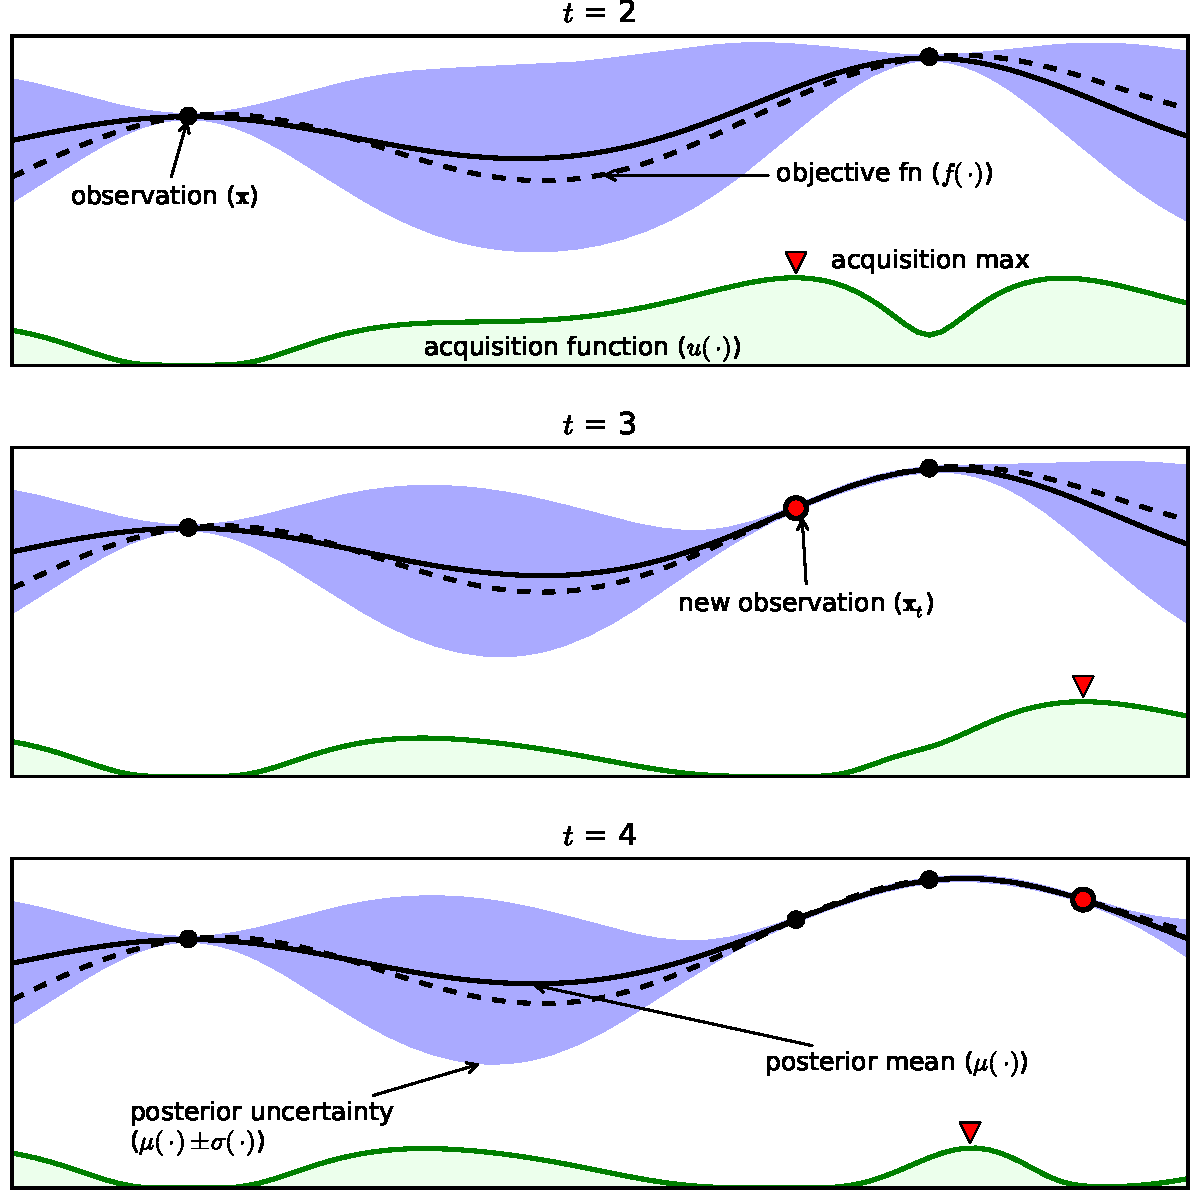
\includegraphics[width=0.85\textwidth]{figures/ml/toyGPtext3.pdf}
\caption{
Illustration of Bayesian optimization over three iterations in a toy 1D maximization problem \cite{Brochu2010}.
Note that the maximum of the acquisition function $u\left(\cdot\right)$
locates where $S\left(\bm{\beta}\right)$ should be sampled next.
The GP estimated posterior distribution of $S\left(\bm{\beta}\right)$
and $u\left(\cdot\right)$ are then updated.
This iterative process is repeated until the estimated maximum is satisfactory.
}
\label{fig:additional:unsupervised:BO:BO_ex}
\end{figure}

%%%%%%%%%%%%%%%%%%%%%%%%%%%%%%%%%%%%%%%%%%%%%%%%%%%%%%%%
\subsection{Gaussian Mixture Model (GMM)}
\label{additional:unsupervised:GMM}
% TODO

%%%%%%%%%%%%%%%%%%%%%%%%%%%%%%%%%%%%%%%%%%%%%%%%%%%%%%%%
\subsection{\texorpdfstring{$\epsilon$}{epsilon}-Means}
\label{additional:unsupervised:epsilonMean}
% TODO

%%%%%%%%%%%%%%%%%%%%%%%%%%%%%%%%%%%%%%%%%%%%%%%%%%%%%%%%
\subsection{Louvain Method}
\label{additional:unsupervised:louvain}
% TODO

%%%%%%%%%%%%%%%%%%%%%%%%%%%%%%%%%%%%%%%%%%%%%%%%%%%%%%%%
\subsection{Variational Autoencoders (VAE)}
\label{additional:unsupervised:VAE}
% TODO

%%%%%%%%%%%%%%%%%%%%%%%%%%%%%%%%%%%%%%%%%%%%%%%%%%%%%%%%
\subsection{Support Vector Clustering}
\label{additional:unsupervised:SVC}
% TODO

